\documentclass[convert={outfile=\jobname.png}]{standalone}
\usepackage{base}
\usepackage{draw}

\begin{document}

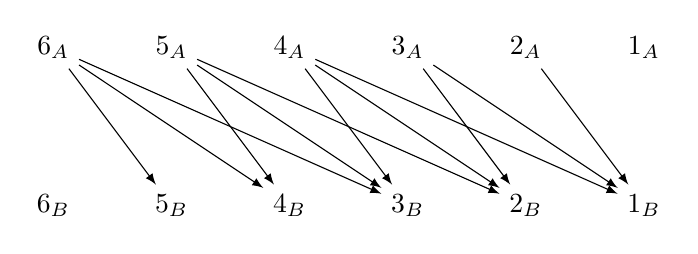
\begin{tikzpicture}
    \foreach \x in {1,...,6} {
        \node (A\x) at (-1.5*\x,0) {$\x_A$};
        \node (B\x) at (-1.5*\x,-2) {$\x_B$};
    }
    \foreach \x in {1,...,5} {
        \draw[->, >=latex] (A\the\numexpr1+\x) -> (B\x);
    }
    \foreach \x in {1,...,4} {
        \draw[->, >=latex] (A\the\numexpr2+\x) to (B\x);
    }
    \foreach \x in {1,...,3} {
        \draw[->, >=latex] (A\the\numexpr3+\x) to (B\x);
    }
\end{tikzpicture}

\end{document}
